\section{Copula表示}
\label{sec:dfam-copulas}

两台设备的寿命$X_1,X_2$都服从$\operatorname{Exp}(1)$。只凭这一点，还说不出两台设备都在一年内损坏的概率：若两台互不影响，它是$(1-\mathrm{e}^{-1})^{2}\approx0.400$；若两台总是同时损坏，它是$1-\mathrm{e}^{-1}\approx0.632$。边缘分布相同，联合分布却可以很不一样。我们想把联合分布中“边缘以外的部分”单独拿出来，作为一个可以与任何边缘搭配的对象。

\subsection{边缘与依赖的分离}
\label{sec:dfam-copula-separation}

把每个分量都换成均匀分布的刻度，各分量自己的规律就被抹掉了，剩下的只有它们怎样一起变化。

\begin{definition}[Copula]
\label{def:dfam-copula}
设随机向量$\bm{U}=(U_1,\dots,U_d)$的每个分量都服从$\operatorname{Unif}(0,1)$。$\bm{U}$的联合分布函数在$[0,1]^{d}$上的限制
\begin{equation}
  C(u_1,\dots,u_d)=\mathbb{P}(U_1\leq u_1,\dots,U_d\leq u_d)
  \label{eq:dfam-copula}
\end{equation}
称为一个Copula。
\end{definition}

Copula就是边缘全为均匀分布的联合分布函数。最简单的三个例子都在$d=2$时看。$U_1,U_2$独立时，
\[
  \Pi(u,v)=uv ,
\]
称为\term{乘积Copula}（product copula）。取一个均匀变量$U$，令$U_1=U_2=U$，两个分量完全同向变化，
\[
  M(u,v)=\mathbb{P}(U\leq u,\ U\leq v)=\min(u,v).
\]
令$U_1=U$、$U_2=1-U$，两个分量完全反向变化，
\[
  W(u,v)=\mathbb{P}(U\leq u,\ 1-U\leq v)=\max(u+v-1,\,0).
\]
另一个常用的例子来自高斯向量。设$(G_1,G_2)$是标准化的二元高斯向量，相关系数为$\rho$。$\Phi$连续且严格增，所以对$0<u<1$，
\[
  \mathbb{P}\bigl(\Phi(G_i)\leq u\bigr)=\mathbb{P}\bigl(G_i\leq\Phi^{-1}(u)\bigr)=u ,
\]
$(\Phi(G_1),\Phi(G_2))$的边缘都是均匀的，它的联合分布函数$C_\rho$称为\term{高斯Copula}（Gaussian copula）。

\paragraph{用Copula拼出联合分布}
给定一个Copula和任意一组边缘分布，可以拼出联合分布。办法是把均匀变量按各自的分位数函数送到目标刻度上，这正是第~\ref{chap:random-variables}章由$\operatorname{Unif}(0,1)$生成任意分布的办法，只是现在$d$个均匀变量带着依赖一起被送过去。这个构造与它的逆向结论合称\term{Sklar定理}（Sklar's theorem）。

\begin{theorem}[Sklar定理]
\label{thm:dfam-sklar}
\begin{enumerate}
  \item 设$C$是$d$元Copula，$F_1,\dots,F_d$是一元分布函数。则
  \begin{equation}
    F(x_1,\dots,x_d)=C\bigl(F_1(x_1),\dots,F_d(x_d)\bigr)
    \label{eq:dfam-sklar}
  \end{equation}
  是一个$d$元联合分布函数，其第$i$个边缘分布函数为$F_i$。
  \item 反之，设$F$是$d$元联合分布函数，边缘分布函数为$F_1,\dots,F_d$。则存在Copula $C$使式~\eqref{eq:dfam-sklar}成立，并且$C$在$\operatorname{Ran}F_1\times\cdots\times\operatorname{Ran}F_d$上由$F$唯一确定，其中$\operatorname{Ran}F_i$是$F_i$的值域。
\end{enumerate}
\end{theorem}

\begin{proof}[第一部分的证明]
设$\bm{U}$的联合分布函数为$C$，$Q_i$为$F_i$的分位数函数，令$X_i=Q_i(U_i)$。每个$U_i$均匀，所以$\mathbb{P}(U_i\in\{0,1\})=0$，下面可以只考虑$U_i\in(0,1)$。第~\ref{chap:random-variables}章的引理给出：对$u\in(0,1)$，
\[
  Q_i(u)\leq x\iff u\leq F_i(x).
\]
于是事件$\{X_i\leq x_i\}$与$\{U_i\leq F_i(x_i)\}$几乎必然相同，对$i=1,\dots,d$同时成立，所以
\[
  \begin{aligned}
    \mathbb{P}(X_1\leq x_1,\dots,X_d\leq x_d)&=\mathbb{P}\bigl(U_1\leq F_1(x_1),\dots,U_d\leq F_d(x_d)\bigr)\\
    &=C\bigl(F_1(x_1),\dots,F_d(x_d)\bigr).
  \end{aligned}
\]
左边是随机向量$(X_1,\dots,X_d)$的联合分布函数，所以式~\eqref{eq:dfam-sklar}是联合分布函数。由同一章的定理，$X_i=Q_i(U_i)$的分布函数是$F_i$，这就是第$i$个边缘。
\end{proof}

第二部分的证明要把一般的$\bm{X}$送回均匀刻度，边缘有没有原子会使做法和结论都不同，留到下一小节。

第一部分已经说明了分离的含义：边缘$F_1,\dots,F_d$与Copula $C$可以独立地选。同一组边缘配上不同的$C$，得到不同的联合分布；同一个$C$配上不同的边缘，依赖的“样式”保持不变。

\paragraph{两台设备}
回到本节开头的两台设备，$F_1=F_2$为$\operatorname{Exp}(1)$的分布函数，$F_1(1)=1-\mathrm{e}^{-1}\approx0.632$。由式~\eqref{eq:dfam-sklar}，两台都在一年内损坏的概率是$C(0.632,0.632)$。代入三个Copula，
\[
  \Pi:\ 0.632^{2}\approx0.400,\qquad M:\ 0.632,\qquad W:\ 2\times0.632-1\approx0.264 .
\]
高斯Copula取$\rho=0.7$时，这个概率是$\mathbb{P}(G_1\leq z,G_2\leq z)$，其中$z=\Phi^{-1}(0.632)\approx0.337$，数值积分得约$0.513$，介于独立与完全同向之间。

图~\ref{fig:dfam-copula-samples}上排是三个Copula的样本，都在单位正方形中；下排把同一批样本用$Q(u)=-\ln(1-u)$送到$\operatorname{Exp}(1)$的刻度上。下排三幅图的两个边缘完全相同，点的排列却各不相同：独立时散成一片，高斯Copula时沿对角线聚集，完全同向时全部落在对角线上。

\begin{BookInlineFigure}
  \centering
  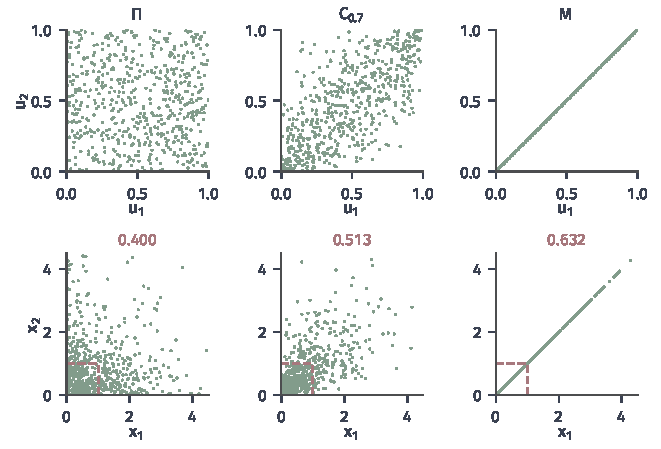
\includegraphics[width=112mm]{figures/07-probability/04-distribution-analysis/matplotlib/dfam-copula-samples/figure.pdf}
  \caption{同样的边缘，不同的依赖。上排：乘积Copula $\Pi$、$\rho=0.7$的高斯Copula、完全同向的$M$，各$600$个样本（绿，种子$716$）。下排：把上排每个点的两个坐标都用$u\mapsto-\ln(1-u)$变换，两个边缘都是$\operatorname{Exp}(1)$；红色虚线围出事件$\{X_1\leq1,X_2\leq1\}$，其概率依次约为$0.400$、$0.513$、$0.632$。}
  \label{fig:dfam-copula-samples}
\end{BookInlineFigure}

\paragraph{依赖的两个极端}
$M$与$W$分别是“完全同向”与“完全反向”的依赖，任何二元Copula都夹在它们之间。

\begin{lemma}[Fréchet–Hoeffding界]
\label{lem:dfam-frechet-bounds}
对任一二元Copula $C$与$u,v\in[0,1]$，
\begin{equation}
  W(u,v)\leq C(u,v)\leq M(u,v).
  \label{eq:dfam-frechet-bounds}
\end{equation}
\end{lemma}

\begin{proof}
设$(U_1,U_2)$的联合分布函数为$C$。事件$\{U_1\leq u,U_2\leq v\}$包含于$\{U_1\leq u\}$，也包含于$\{U_2\leq v\}$，所以$C(u,v)\leq u$且$C(u,v)\leq v$，即$C\leq M$。另一方面，由并集的概率公式，
\[
  C(u,v)=\mathbb{P}(U_1\leq u)+\mathbb{P}(U_2\leq v)-\mathbb{P}(U_1\leq u\text{或}U_2\leq v)\geq u+v-1 ,
\]
又$C(u,v)\geq0$，所以$C\geq W$。
\end{proof}

图~\ref{fig:dfam-copula-bounds}沿对角线比较几个Copula：$C(u,u)$是两个分量都不超过各自$u$分位数的概率。完全同向时它等于$u$，独立时是$u^{2}$，完全反向时在$u\leq1/2$以前一直为零。图中$u=0.632$处的四个值就是上面两台设备的四个概率。

\begin{BookInlineFigure}
  \centering
  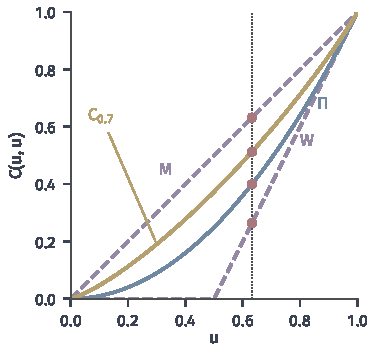
\includegraphics[width=64mm]{figures/07-probability/04-distribution-analysis/matplotlib/dfam-copula-bounds/figure.pdf}
  \caption{Copula在对角线上的取值$C(u,u)$。紫色虚线为上下界$M(u,u)=u$与$W(u,u)=\max(2u-1,0)$，蓝线为乘积Copula $u^{2}$，黄线为$\rho=0.7$的高斯Copula。红点标出$u=1-\mathrm{e}^{-1}\approx0.632$处的四个值$0.264,0.400,0.513,0.632$。}
  \label{fig:dfam-copula-bounds}
\end{BookInlineFigure}

\subsection{唯一性的范围}
\label{sec:dfam-copula-uniqueness}

现在反过来：给定$\bm{X}$的联合分布，能否找到它的Copula，找到的是否唯一？自然的想法是把每个分量用自己的分布函数送回$(0,1)$，令$U_i=F_i(X_i)$。这个想法在边缘连续时完全成立，在边缘有原子时会出问题。

\paragraph{连续边缘：概率积分变换}
先看一个分量。把$X$代入它自己的分布函数，得到$F(X)$，这个操作称为\term{概率积分变换}（probability integral transform）。

\begin{lemma}[概率积分变换]
\label{lem:dfam-pit}
设实值随机变量$X$的分布函数$F$连续。则$F(X)\sim\operatorname{Unif}(0,1)$，并且对每个$x$，事件$\{F(X)\leq F(x)\}$与$\{X\leq x\}$只差一个零概率事件。
\end{lemma}

\begin{proof}
记$Q$为$F$的分位数函数。对$u\in(0,1)$，由第~\ref{chap:random-variables}章的引理，$F(y)\geq u$当且仅当$y\geq Q(u)$，所以
\[
  \mathbb{P}\bigl(F(X)\geq u\bigr)=\mathbb{P}\bigl(X\geq Q(u)\bigr)=1-F\bigl(Q(u)-\bigr).
\]
另一方面，由同一引理有$F(Q(u))\geq u$；对$y<Q(u)$又有$F(y)<u$，令$y\uparrow Q(u)$得$F(Q(u)-)\leq u$。$F$连续，左极限等于函数值，两者合起来给出$F(Q(u))=u$。代入上式，
\[
  \mathbb{P}\bigl(F(X)\geq u\bigr)=1-u ,
\]
所以$F(X)$在$(0,1)$上均匀，又以概率$1$取值于$[0,1]$。

对第二个结论，$\{X\leq x\}\subseteq\{F(X)\leq F(x)\}$由单调性得到。差集是$\{X>x,\ F(X)=F(x)\}$，在其上$X$落在$F$取常值$F(x)$的区间里。记$b=\sup\{y:F(y)=F(x)\}$，这个事件包含于$\{x<X\leq b\}$（$b=+\infty$时为$\{X>x\}$），其概率是$F(b)-F(x)=0$（$b$有限时$F$连续，$F(b)=F(x)$；$b=+\infty$时$F(x)=1$）。
\end{proof}

\begin{proof}[Sklar定理第二部分的证明（边缘连续）]
设各$F_i$连续，令$U_i=F_i(X_i)$，$C$为$\bm{U}$的联合分布函数。由引理~\ref{lem:dfam-pit}，每个$U_i$均匀，$C$是Copula；且$\{U_i\leq F_i(x_i)\}$与$\{X_i\leq x_i\}$只差零概率事件，所以
\[
  C\bigl(F_1(x_1),\dots,F_d(x_d)\bigr)=\mathbb{P}(X_1\leq x_1,\dots,X_d\leq x_d)=F(x_1,\dots,x_d).
\]
唯一性：若$C'$也满足式~\eqref{eq:dfam-sklar}，则对每组$x_i$有$C'(F_1(x_1),\dots)=F(x_1,\dots)=C(F_1(x_1),\dots)$，所以$C'$与$C$在$\operatorname{Ran}F_1\times\cdots\times\operatorname{Ran}F_d$上相等。$F_i$连续时值域包含$(0,1)$，再由下面的引理~\ref{lem:dfam-copula-lipschitz}，$C$与$C'$都连续，于是在$[0,1]^{d}$上处处相等。
\end{proof}

\begin{lemma}[Copula的Lipschitz性]
\label{lem:dfam-copula-lipschitz}
对任一$d$元Copula $C$与$\bm{u},\bm{v}\in[0,1]^{d}$，
\begin{equation}
  \lvert C(\bm{u})-C(\bm{v})\rvert\leq\sum_{i=1}^{d}\lvert u_i-v_i\rvert .
  \label{eq:dfam-copula-lipschitz}
\end{equation}
\end{lemma}

\begin{proof}
设$\bm{U}$的联合分布函数为$C$。事件$\{\bm{U}\leq\bm{u}\}$与$\{\bm{U}\leq\bm{v}\}$的对称差中，至少有一个$i$使$U_i$落在$u_i$与$v_i$之间。由并集的概率不超过概率之和，
\[
  \lvert C(\bm{u})-C(\bm{v})\rvert\leq\sum_{i=1}^{d}\mathbb{P}\bigl(\min(u_i,v_i)<U_i\leq\max(u_i,v_i)\bigr)=\sum_{i=1}^{d}\lvert u_i-v_i\rvert ,
\]
最后一步用到$U_i$均匀。
\end{proof}

边缘连续时，唯一的Copula还有一个有用的性质。证明表明，这个Copula就是$(F_1(X_1),\dots,F_d(X_d))$的联合分布函数。设$g_1,\dots,g_d$都严格递增，$Y_i=g_i(X_i)$，其分布函数记为$G_i$。由$\{Y_i\leq g_i(x)\}=\{X_i\leq x\}$，
\[
  G_i\bigl(g_i(x)\bigr)=F_i(x),
\]
$G_i$也连续（$\mathbb{P}(Y_i=y)$不超过$X_i$取某个单点的概率，为零）。于是$G_i(Y_i)=F_i(X_i)$，$(Y_1,\dots,Y_d)$送回均匀刻度后得到的是同一个随机向量，Copula相同。分量各自作严格递增的重新刻度，Copula不变；依赖结构因此与单位、对数刻度这类选择无关，这正是“边缘以外的部分”应有的样子。

\paragraph{有原子时只在值域上唯一}
边缘有原子时，概率积分变换失效。取$X\sim\operatorname{Bern}(\tfrac12)$，$F(0)=\tfrac12$，$F(1)=1$，于是$F(X)$只取$\tfrac12$和$1$两个值，各有概率$\tfrac12$，根本不是均匀分布。图~\ref{fig:dfam-pit}(b)画出了这一点：质量在原子处不能被摊开；作为对照，(a)中连续的$\operatorname{Exp}(1)$经概率积分变换后确实均匀。

\begin{BookInlineFigure}
  \centering
  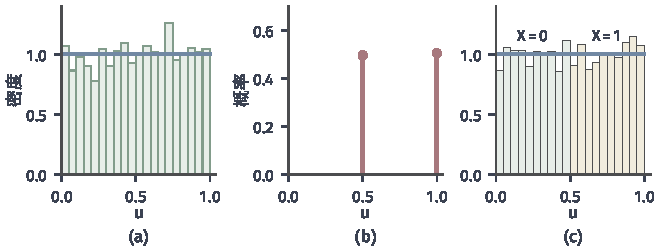
\includegraphics[width=112mm]{figures/07-probability/04-distribution-analysis/matplotlib/dfam-pit/figure.pdf}
  \caption{把分量送回均匀刻度，各$4000$个模拟值（种子$716$）。(a)$X\sim\operatorname{Exp}(1)$时$F(X)$的直方图（浅绿），蓝线是均匀密度$1$。(b)$X\sim\operatorname{Bern}(\frac12)$时$F(X)$只取$\frac12$与$1$（红色竖线，高度为概率）。(c)同一枚硬币的分布变换$U=F(X-)+V\Delta F(X)$：$X=0$的值摊在$(0,\frac12]$（浅绿），$X=1$的值摊在$(\frac12,1]$（浅黄），合起来是均匀分布。}
  \label{fig:dfam-pit}
\end{BookInlineFigure}

再看唯一性。设$X_1,X_2$是两枚独立的公平硬币。$\operatorname{Ran}F_i=\{0,\tfrac12,1\}$，式~\eqref{eq:dfam-sklar}只在这九个格点上约束$C$。$u$或$v$为$0$时任何Copula都取$0$，$u=1$时取$v$，$v=1$时取$u$，这些格点自动满足；真正的约束只有一个：
\[
  C(\tfrac12,\tfrac12)=\mathbb{P}(X_1=0,X_2=0)=\tfrac14 .
\]
乘积Copula满足它。$C'=\tfrac12M+\tfrac12W$也满足：两个Copula的凸组合仍是Copula（按权重混合两个均匀边缘的随机向量，边缘仍均匀），且
\[
  C'(\tfrac12,\tfrac12)=\tfrac12\cdot\tfrac12+\tfrac12\cdot0=\tfrac14 .
\]
可是在$(\tfrac14,\tfrac14)$处，$\Pi$取$\tfrac1{16}$，$C'$取$\tfrac12\cdot\tfrac14+0=\tfrac18$，两者不同。所以两枚独立硬币的联合分布既可以写成$\Pi(F_1,F_2)$，也可以写成$C'(F_1,F_2)$。

\begin{BookInlineFigure}
  \centering
  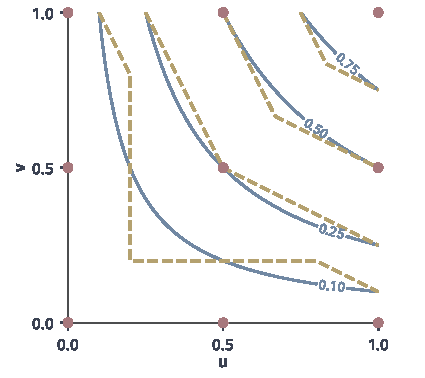
\includegraphics[width=72mm]{figures/07-probability/04-distribution-analysis/matplotlib/dfam-copula-atoms/figure.pdf}
  \caption{有原子时Copula只在值域格点上确定。两枚独立公平硬币，$\operatorname{Ran}F_1\times\operatorname{Ran}F_2$是九个格点（红点）。蓝色实线是乘积Copula $\Pi$的等值线，黄色虚线是$\frac12M+\frac12W$的等值线，层级为$0.1,0.25,0.5,0.75$；两族曲线在红点处取相同的值，在格点之间不同。}
  \label{fig:dfam-copula-atoms}
\end{BookInlineFigure}

图~\ref{fig:dfam-copula-atoms}画出这两个Copula的等值线：它们在九个红点上一致，在其他地方不同。这个例子说明，含原子时“从联合分布读出的Copula”并不唯一，不同的选择可能给人截然不同的依赖印象：$C'$看上去一半完全同向、一半完全反向，实际描述的却是两枚独立的硬币。连续情形的变换论证不能照搬，依据Copula谈论依赖时，必须先确认边缘是否连续。

\paragraph{有原子时的存在性}
唯一性失去了，存在性仍然成立。办法是在每个原子上用一个独立的均匀变量把质量摊开，这称为\term{分布变换}（distributional transform）。

\begin{lemma}[分布变换]
\label{lem:dfam-distributional-transform}
设$X$的分布函数为$F$，$V\sim\operatorname{Unif}(0,1)$与$X$独立，记$F(x-)$为左极限、$\Delta F(x)=F(x)-F(x-)$。令
\begin{equation}
  U=F(X-)+V\,\Delta F(X).
  \label{eq:dfam-distributional-transform}
\end{equation}
则$U\sim\operatorname{Unif}(0,1)$，并且对每个$x$，事件$\{U\leq F(x)\}$与$\{X\leq x\}$只差一个零概率事件。
\end{lemma}

\begin{proof}
固定$u\in(0,1)$，令$x_0=Q(u)$，则$F(x_0-)\leq u\leq F(x_0)$。由$V$与$X$独立，给定$X=y$时$U$在区间$[F(y-),F(y)]$上均匀（$\Delta F(y)=0$时退化为一点），所以
\[
  \mathbb{P}(U\leq u)=\mathbb{E}[g(X)],\qquad g(y)=\mathbb{P}\bigl(F(y-)+V\Delta F(y)\leq u\bigr).
\]
按$y$与$x_0$的位置分三种情形：
\begin{itemize}
  \item $y<x_0$：$F(y)\leq F(x_0-)\leq u$，$g(y)=1$，这部分贡献$\mathbb{P}(X<x_0)=F(x_0-)$。
  \item $y=x_0$：若$\Delta F(x_0)>0$，$g(x_0)=(u-F(x_0-))/\Delta F(x_0)$，贡献$\Delta F(x_0)\,g(x_0)=u-F(x_0-)$；若$\Delta F(x_0)=0$，则$F(x_0-)=u$，贡献为$0=u-F(x_0-)$。
  \item $y>x_0$：$F(y-)\geq F(x_0)\geq u$。$g(y)>0$只可能在$F(y-)=u$且$\Delta F(y)=0$时发生，这时$F(y)=F(x_0)$，$y$落在$F$取常值的区间里，这样的$y$整体的概率为零（与引理~\ref{lem:dfam-pit}的论证相同），贡献为$0$。
\end{itemize}
三部分相加，
\[
  \mathbb{P}(U\leq u)=F(x_0-)+\bigl(u-F(x_0-)\bigr)=u ,
\]
所以$U$均匀。

对第二个结论，$X\leq x$时$U\leq F(X)\leq F(x)$。$X>x$时$U\geq F(X-)\geq F(x)$，要使$U\leq F(x)$只能$U=F(x)=F(X-)$且$V\Delta F(X)=0$，即$V=0$，或者$\Delta F(X)=0$而$F(X)=F(x)$；前者概率为零，后者又是$X$落在$F$取常值的区间里，概率也为零。
\end{proof}

\begin{proof}[Sklar定理第二部分的证明（一般情形）]
取与$\bm{X}$独立的$V_1,\dots,V_d$，它们独立同分布于$\operatorname{Unif}(0,1)$，对每个分量按式~\eqref{eq:dfam-distributional-transform}作分布变换，得到$\bm{U}$，令$C$为它的联合分布函数。由引理~\ref{lem:dfam-distributional-transform}，$C$是Copula，且$\{U_i\leq F_i(x_i)\}$与$\{X_i\leq x_i\}$只差零概率事件，与连续情形一样得到式~\eqref{eq:dfam-sklar}。在$\operatorname{Ran}F_1\times\cdots\times\operatorname{Ran}F_d$上的唯一性，与连续情形的论证相同。
\end{proof}

分布变换在连续点上退化为$F(X)$，所以它是概率积分变换的推广。它得到的Copula依赖于为摊开原子而引入的独立变量$V_i$：图~\ref{fig:dfam-pit}(c)中，硬币的两个原子各被摊成长为$\tfrac12$的一段，两枚独立硬币配独立的$V_1,V_2$，得到的正是乘积Copula；若让$V_1=V_2$，就得到另一个同样合法的Copula。这再次说明含原子时Copula是联合分布的一种表示，而不是由它唯一决定的量。
